\hypertarget{ux4ebaux529bux6295ux8d44}{%
\subsubsection{人力投资}\label{ux4ebaux529bux6295ux8d44}}

问题:组织投入人力对社区所做的贡献(例如:代码提交,议题和更改请求)花费的成本是多少

\hypertarget{ux63cfux8ff0}{%
\paragraph{描述}\label{ux63cfux8ff0}}

开源项目通常由组织的人力投入来支撑。该指标跟踪组织对单个项目的经济投入(体现在人力成本)。

\hypertarget{ux76eeux6807}{%
\paragraph{目标}\label{ux76eeux6807}}

随着组织参与度对开源项目变得越来越重要,组织必须清楚了解其人力投资。该指标的目的是为从事开源项目的组织提高人力成本的透明度。该指标给开源项目办公室(OSPO)经理提供了一种通过项目投资组合比较人力成本的方法。比如:人力投资指标能用在确定投资的优先顺序或者确定投资回报。例如:

\begin{itemize}
\tightlist
\item
  以人力投资评估 OSPO 事务的优先级和证明预算合理性
\item
  以人力投资解释产品、项目管理事项的优先级
\item
  以人力投资论证继续投资 OSPO 的价值
\item
  以人力投资反应和比较开源贡献与内部工作的人力成本
\item
  以人力投资比较项目组合的项目效益
\end{itemize}

\hypertarget{ux5b9eux73b0}{%
\paragraph{实现}\label{ux5b9eux73b0}}

基础指标包括:

\begin{itemize}
\tightlist
\item
  贡献数量
\item
  按贡献者类型(内部/外部)划分的贡献数量
\item
  按贡献类型(如代码提交,议题和更改请求)划分的贡献数量
\end{itemize}

参数包括:

\begin{itemize}
\tightlist
\item
  每小时劳动率
\item
  创建贡献的平均劳动时间(按照贡献类型分类)
\end{itemize}

人力投资 = 每一种贡献类型的总和(贡献数量 * 创造贡献的平均工时 *
平均每小时劳动率)

\hypertarget{ux7b5bux9009ux6761ux4ef6}{%
\subparagraph{筛选条件}\label{ux7b5bux9009ux6761ux4ef6}}

\begin{itemize}
\tightlist
\item
  内部与外部贡献者
\item
  问题标签
\item
  项目来源(如内部、开源仓库、竞争对手的开源仓库)
\end{itemize}

\hypertarget{ux53efux89c6ux5316ux6548ux679c}{%
\subparagraph{可视化效果}\label{ux53efux89c6ux5316ux6548ux679c}}

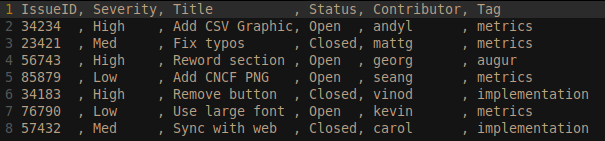
\includegraphics{images/labor-investment_csv.png}

我们的第一个参数化指标的可视化效果依赖于可以用Augur导出的CSV。电子表格用于指标参数和计算公式。未来的实现可能会在
webapp 中直接添加参数操作的功能。

\hypertarget{ux53c2ux8003ux8d44ux6599}{%
\paragraph{参考资料}\label{ux53c2ux8003ux8d44ux6599}}

\begin{itemize}
\tightlist
\item
  \href{https://www.slideshare.net/caniszczyk/starting-an-open-source-program-office-ospo}{启动开源项目办公室}
\item
  \href{https://events19.linuxfoundation.org/wp-content/uploads/2018/07/OSLS_2019-untold-story-of-OSPO.pdf}{创办开源项目办公室}
\item
  \href{https://d1.awsstatic.com/Open\%20Source/enterprise-oss-book.pdf}{企业开源}
\end{itemize}
